\documentclass[10pt,twocolumn,twoside]{pnas-new}
% Use the lineno option to display guide line numbers if required.
% Note that the use of elements such as single-column equations
% may affect the guide line number alignment.

\templatetype{pnasmathematics} % Choose template
% {pnasresearcharticle} = Template for a two-column research article
% {pnasmathematics} = Template for a one-column mathematics article
% {pnasinvited} = Template for a PNAS invited submission

\usepackage[utf8]{inputenc}
\usepackage[english]{babel}
\usepackage{amsmath,amsthm,amssymb,enumerate,euscript,mathrsfs}

\newtheorem{theorem}{Theorem}[section]
\newtheorem{corollary}{Corollary}[theorem]
\newtheorem{lemma}[theorem]{Lemma}


\title{A Collection of Thoughts on the Keccak/SHA-3 Construction}

% Use letters for affiliations, numbers to show equal authorship (if applicable) and to indicate the corresponding author
\author{Alexander Scheel}

\affil{Iowa State University}

% Please give the surname of the lead author for the running footer
\leadauthor{Scheel}

% Please add here a significance statement to explain the relevance of your work

% Please include corresponding author, author contribution and author declaration information
\correspondingauthor{E-mail: alexander.m.scheel\@gmail.com}

% Keywords are not mandatory, but authors are strongly encouraged to provide them. If provided, please include two to five keywords, separated by the pipe symbol, e.g:

\begin{abstract}
    In this paper, we discuss new techniques for the cryptanalysis of
    Keccak/SHA-3, though none of the resulting attacks scale to full versions
    of the hash function. We show an explicit construction for the inverses of
    the core round functions, the permutation orders of the round functions,
    and an attack which exploits low-order cycles. Further, we introduce new
    logical cryptanalysis techniques and show the existence of partial fixed
    points to produce 2-1 block collisions.
\end{abstract}

\keywords{MATH 490 $|$ Advisor: Dr. Clifford Bergman $|$ SHA-3 $|$ hash\_framework }

\begin{document}

% Optional adjustment to line up main text (after abstract) of first page with line numbers, when using both lineno and twocolumn options.
% You should only change this length when you've finalised the article contents.
\verticaladjustment{-2pt}

\maketitle
% \thispagestyle{firststyle}
% \ifthenelse{\boolean{shortarticle}}{\ifthenelse{\boolean{singlecolumn}}{\abscontentformatted}{\abscontent}}{}

% Bibliography
% \bibliography{pnas-sample}

\section{A Series of Introductions} \label{sec:intro}
    This paper presents the work of the author towards the completion of the
requirements for the MATH 490 Independent Study course under Dr. Clifford
Bergman at Iowa State University of Science and Technology. This work was an
extension of the author's Honors Project under Dr. Eric Davis and utilized
the resulting
\href{https://github.com/cipherboy/hash\_framework}{hash\_framework} project
(viewable under the \texttt{cipherboy} account on GitHub.com).
Additional artifacts related to this project can be seen in the
\href{https://github.com/cipherboy/keccak-attacks}{keccak-attacks} repository.
A permanent location for this document is in the
\href{https://github.com/cipherboy/papers}{papers} repository.

    Within this section are a series of introductions which provide necessary
background on the topics of cryptographic hash functions, the development of
Keccak/SHA-3, and its structure. While certain sections can be skipped if the
reader has the prerequisite knowledge, hopefully all readers find the material
engaging and useful. Following these introductions, this paper presents the
analysis of the Keccak/SHA-3 hash function before concluding with a final
evaluation and further work.

    The remaining sections outside of the introductions discuss 1) various
mathematical properties of the core round functions, 2) exhaustive collision
searches on small instances, 3) correlation matrices, and 4) fixed point
attacks.

% TODO
% More information about structure of analysis section.

% TODO Outline
%    - Historic
%        - Ciphers vs Codes
%
%    - Modern
%        - Symmetric
%        - Asymmetric
%        - Hash Functions
%        - Building Protocols

\subsection{Introduction on the Topics of Cryptographic Hash Functions} \label{sec:i:hash}

    While there are many applications of pure mathematics, few are as
demanding and shrouded in secrecy as cryptography. Cryptography exists
because of the fundamental need of civilizations, governments, and individuals
to keep secrets secure from devoted adversaries. While modern cryptography
combines the disciplines of mathematics, computer science, and computer
engineering, prior to the turn of the 20th century, cryptography lacked much
of its modern rigor.

    Within cryptography's collection of algorithms, few are as useful as
hash functions have proven to be to cryptographers and non-cryptographers
alike. A hash function maps arbitrary length binary strings to binary strings
of a fixed length; typically we denote such a function $h$. Because the inputs
are of arbitrary size, by the pigeonhole principle, there must exist at least
one collision: two blocks $x \neq y$ such that $h(x) = h(y)$. However, to be
considered cryptographically secure, finding such a collision must be hard
(on the order of $2^{\frac{b}{2}}$ for $b$ the number of bits in the output).

    Further, a cryptographic hash function must be resistant finding a
preimage: for a given output value $v$, finding an input $x$ such that
$h(x) = v$ should be roughly on the order of $2^{b}$. Given such an attack,
it is possible to find a collision: choose a random input, compute its hash,
then use the preimage attack to find a different input for that hash; these two
inputs form a collision pair. Thus a preimage attack is stronger than a
collision attack.

    However, if the attacker is allowed to choose only one message (that is,
the challenger chooses the other), this forms a second preimage attack. More
formally, for a given fixed message $x$, the attacker seeks a $y \neq x$ such
that $h(x) = h(y)$. While a collision attack is only valid for some such
messages, $x$, a preimage attack has to be valid for all such $x$; thus it is
a stronger attack than collision attacks, but weaker than a preimage attack
as it presupposes an existing message.

\subsection{Introduction on the Usages of Hash Functions}

    Studying the integrity of hash function is important because hash functions
are a fundamental building block of both cryptographic and non-cryptographic
systems. While a body of literature developed around attacking the previous
hash functions (of MD4, MD5, SHA-1 and SHA-2), many of these attacks do not
directly translate to Keccak/SHA-3 because its construction differs
substantially. Further, many of these attacks started only as generic attacks
with low utility, and only with substantial work, were they translated to
highly specialized attacks on specific use cases. Below is a discussion of
various places where cryptographic hash functions are used, and what types of
attacks they are most susceptible to.

    The most common use case for hash functions are in signatures. Often times
the cryptography underlying asymmetric signatures (where one party can sign a
message and any party can verify that the signature and message is authentic)
can only sign fixed length messages, often only in the thousands of bytes.
However, longer data frequently must be signed. Thus, most implementations of
signature schemes use a cryptographically secure hash function and sign the
digest instead of the actual message. This can be seen in PGP, TLS, and PKI.
Often, these implementations are most vulnerable to a second preimage attack,
as one message is already provided. However, when the attacker has control
over both messages, a collision attack will suffice.

    Another common use case for hash functions are in message integrity
verification. In this case, a hash of the message is sent along side of the
message to ensure that the message hasn't been tampered with. While often this
signature should be signed, it is frequently used in cases where the
authenticity of the hash isn't questioned. This includes verifying contents of
files on disk or in version control systems such as Git. In both of these
cases, second preimage and collision attacks are the most useful for an
attacker.

\subsection{Introduction on the Scope of the Independent Study}

    This independent study focused on a single hash function, Keccak, which
was chosen by NIST to be the next standardized algorithm, SHA-3 \cite{NIST202}.
This hash function differs from previously standardized algorithms in two major
ways: one, it is not based on the Merkel-Damg{\aa}rd construct and is rather
based on the Sponge construction, and two, the internal round function is not a
compression function and is instead a permutation. Outside of a few theorems
done by hand and verifying the lack of low-order correlations, we focused on
using automated tools to learn more about the structure of SHA-3.

    In the late 1990s, F. Massacci started analyzing cryptographic
constructions using Boolean Satisfability \cite{CryptoSAT}; however, applying
this to hash functions is a largely understudied field. E. Homsirikamol tried
brute forcing collisions in SHA-3 to limited results \cite{Homsirikamol2012},
and P. Morawiecki performed similar work for preimages \cite{cryptoeprint:2010:285}.
However, neither contributed useful, general cryptanalysis techniques to scale
attacks against reduced rounds (and reduced sizes) to larger numbers of rounds.
Our work begins exploring new techniques and several consequences in the
following sections.

% TODO Outline
%   - Properties
%   - History of Development
%   - History of Attacks
%   - Modern Theory and Structure


\subsection{Introduction to Terminology} \label{sec:i:terminology}

This section contains a collection terminology useful for discussing SHA-3
and Boolean Satisfiability.

We define $\Sigma = \{0, 1\}$ to be the alphabet.

We define the set $W = \{1, 2, 4, 8, 16, 32, 64\}$ to be the powers of two
typically used in constructing the Keccak widths; $w=64$ is standardized for
use in SHA-3, though any power of two can be used.

For a given $w \in W$, we define $S_{w} = \Sigma^{25w}$, to be the set of
all binary strings of length $25w$; these represent the possible states (which
are binary strings that map onto an indexible array $A$ described later) and each
round permutation maps $S_{w} \mapsto S_{w}$.

A binary string $s \in S_{w}$ can be indexed directly (in a zero-indexed
manner, i.e., the starting bit of $s$ is denoted $s[0]$), or via a 3
dimensional structure of size 5 by 5 by $w$. This is typically done in
conjunction with an uppercase letter, $A = s$, and then
$A[x, y, z] = s[w(5y + x) + z]$. This is in accordance with
FIPS 202 \cite{NIST202}.

\subsection{Introduction on the Development of Keccak/SHA-3} \label{sec:i:keccak}

    NIST standardized Keccak as SHA-3 in FIPS 202 \cite{NIST202}; Keccak was
chosen as the winner of the corresponding hash function design competition
started in 2009. Designed by the Keccak Team (G. Bertoni, J. Daemen, M.
Peeters, G. Van Assche, and R. Van Keer \cite{KeccakTeam}), Keccak features a
novel construction.

    Keccak is built around the concept of a state cube: a 5 by 5 by $w$ cube
of bits (where $w$ is a power of 2). By increasing $w$, a higher security
margin can be given, at the expense of increasing the computational intensity.
However, because internal round operations on this state cube are bijective,
it can be implemented efficiently in hardware with minimal gate and propagation
delays. Typically this state is called $A$ when represented as a cube, and $s$
when represented as a (flat) bit string. There are five major functions which
compose to form a single round: $\theta$, $\rho$, $\pi$, $\chi$, and $\iota$;
each maps bijectively over the entire state space (i.e., elements of
$2^{25w}$).

    $\theta$ is an eleven way XOR and is thus a linear map. For all
$0 \leq x \leq 4$ and $0 \leq z < w$, define:
\begin{align*}
    C[x, z] & := \bigoplus_{0 \leq y \leq 4} A[x, y, z] \\
    D[x, z] & := C[(x-1) \text{ mod } 5, z] \oplus C[(x+1) \text{ mod } 5, (z - 1) \text{ mod } w] \\
\end{align*}
Then:
\begin{align*}
    A'[x, y, z] & := A[x, y, z] \oplus D[x, z]
\end{align*}

    $\rho$ is a pure permutation function, permuting the locations of bits in
a lane (the $z$ component) of the state cube. For all
$0 \leq z < w: A'[0, 0, z] := A[0, 0, z]$. Then let $(x, y) = (1, 0)$, and for
$0 \leq t \leq 23$:
\begin{align*}
    \forall 0 \leq z < w: A'[x, y, z] & := A[x, y, (z - \frac{(t+1)(t+2)}{2}) \text{ mod } w] \\
    \text{ let } (x, y) & = (y, (2x + 3y) \text{ mod } 5)
\end{align*}

    $\pi$ is another pure permutation function, permuting locations along the
face of the cube. For all $0 \leq x \leq 4, 0 \leq y \leq 4, 0 \leq z < w$:
\begin{align*}
    A'[x, y, z] := A[(x + 3y) \text{ mod } 5, x, z].
\end{align*}

    $\chi$ is the only non-linear function and is of degree two (with inverse
of degree three). For all $0 \leq x \leq 4, 0 \leq y \leq 4, 0 \leq z < w$:
\begin{align*}
    A'[x, y, z] := A[x, y, z] \oplus (\lnot A[(x + 1) \text{ mod } 5, y, z] \land A[(x + 2) \text{ mod } 5, y, z]).
\end{align*}

    $\iota$ is a fixed-value XOR useful for preventing trivial fixed points,
and is the only function dependent on the current round number. Refer to
page 16 of FIPS 202 (\cite{NIST202}) for its specification; it is not discussed
extensively in this paper. It takes an additional parameter, $c$, the current
round number.

    The a single round of the core round function function, $r$ is defined as
follows:
\begin{align*}
    r(A, c) = \iota(\chi(\pi(\rho(\theta(A)))), c)
\end{align*}
And the entire core round function, \texttt{KECCAK-$f$}, is thus:
\begin{align*}
    \text{\texttt{KECCAK-$f$}}(A) = r(r( ...  r(A, 0) ... , 22), 23)
\end{align*}

    The sponge construction can be described as follows. Fix $w$ as a power of
two in $W$. Then define a state, $s$, as above to be a binary string of length
$25w$. Fix a security margin $m$ (usually 228, 256, 384, or 512 bits in the
SHA-3 standard). Define $i_{m} = 25w - 2m$ be the input margin, and
$o_{m} = 2m$ be the output margin. For a message $M$, assume it is padded
to a multiple of $i_{m}$ bits according to the scheme in FIPS 202
(\texttt{pad10*1}). Start with initial state $s_0 = 0^{25w}$. For each block
$M_{i}$, XOR $M_{i}$ into the first $|M_{i}|$ bits of state $s_i$ and define:
\begin{align*}
    s_{i+1} = \text{\texttt{KECCAK-$f$}}(s_{i} \oplus M_{i})
\end{align*}
Then if $s_{k}$ is the final state, take the first $m$ bits ($s_{k}[0..m]$)
as the output digest. Additionally if more than $2m$ bits are required, take
the first $2m$ bits, then compute $s_{k+1} = \text{\texttt{KECCAK-$f$}}(s_{k})$
and continue taking at most the first $2m$ bits from $s_{k+1}$, repeating as
necessary. This is demonstrated in Figure \ref{f:s}.

\begin{figure*}
\begin{center}
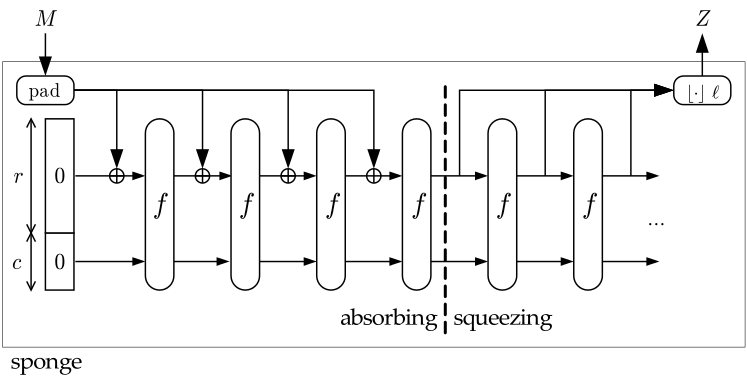
\includegraphics[width=0.7\textwidth]{figs/Sponge-150.png}
\caption{Graphical description of the sponge construction. Courtesy of the
\href{https://keccak.team/images/Sponge-150.png}{Keccak Team}.}
\label{f:s}
\end{center}
\end{figure*}

To have a security margin of $m$ bits, the output needs to have $m$ bits;
however, if the attacker has complete control of all $25w$ bits of state,
they would be able to choose an output with prefix $m$ easily because
Keccak is bijective with a known, computable inverse. Thus, by restricting
the initial state to have a suffix of $2m$ bits of zeros, the attacker must
not only restrict the output to have the correct prefix, but also the input
to have the correct suffix. In this way, the authors claim that Keccak/SHA-3
has collision resistance equal to preimage resistance; finding a collision
is of equivalent difficulty as finding a preimage, and thus Keccak/SHA-3 is
more secure than necessary \cite{Keccak3}.

Further, SHA-3 is secure from trivial multiple-block collisions due to the
restriction of allowing $i_{m}$-bits of input state to be changed directly
via a block. Thus, for a multiple-block collision attack to be possible, the
remaining $25w - i_{m} = 2m$ bits must be the same between the internal state
of a collision pair, allowing two different blocks $b$ and $b'$ to cancel
their initial prefix differences. All of these attacks are constrained
input/output problems and thus reduce to SAT; thus, considerable work
is required to successfully perform an attack.

% TODO Outline
%    - Authors Background (keccak team)
%    - Function design goals
%    - NIST Contest
%    - NIST standardization controversy? (sources?)


%\subsection{Introduction to the Remaining Sections}



%\subsection{Introduction on the Structure of SHA-3} \label{sec:i:structure}

%    SHA-3 consists of two parts: a core permutation function, KECCAK-$f$, and
%a domain extender, the KECCAK sponge function. As discussed by the Keccak
%uthors, additional security is given by choosing the permutation functions to
%be bijective, though they need not be (the domain need only be $S_{w}$).


% TODO Outline
%   - Sponge Function
%   - State Array
%   - Five functions
%   - Keccak-$f$





\section{Mathematical Properties of the Five Round Functions} \label{sec:properties}

In the following section, we detail various mathematical properties of the five
permutation functions which make up the core round function of Keccak. In most
cases, we seek to provide mathematical proofs of these properties. In all
cases, we rely on external code and Boolean Satisfiability for computerized
proofs where proofs are not directly provided. We do note the introduction of
a cleaner form of $\chi^{-1}$ than in existing literature.

% TODO Outline
%   - Outline following subsections

\subsection{Of $\theta$} \label{sec:p:t}

% TODO Outline
%   - Theta -> XOR with 11 different values; linear equations?
%   - What sizes are bijective?
%   - Discussion in literature

In this section, we show that $\theta$ is bijective, that XOR distributes
through $\theta$, give a method for finding the inverse of $\theta$, and
give the order of $\theta$.

Let $w$ be a fixed power of 2. Since $S_{w}$ is of finite size, it suffices to
show that, $\forall x, y \in S_{w}$,
$x \neq y \Rightarrow \theta(x) \neq \theta(y)$. Assume the hypothesis: then
$x \oplus y \neq 0^{25w}$.

\begin{lemma} \label{lem:p:t:1}
\begin{align*}
    \theta(a) = 0^{25w} \iff a = 0^{25w}
\end{align*}
\end{lemma}
\begin{proof}

First, note that $\theta(0^{25w}) = 0^{25w}$ due to construction of $\theta$
having an even number of XORs. Suppose that there existed some other input, x,
to $\theta$ such that $\theta(x) = 0^{25w}$. Note that, $x$ with odd number of
$1$s (that is, $|\{ i : x_{i} = 1 \}| \equiv 1 \text { mod } 2$), $\theta(x)$
likewise has an odd number of ones due to $\theta$ having an even number of
XORs. Similarly, for any $x$ with has an even but non-zero number of ones,
then there exists index $(i, j, k)$ such that $\theta(x)[i, j, k] = 1$. This is
because, for any pair of indices $(i, j, k)$ and $(i', j', k')$ such that
$x[i, j, k] = 1 = x[i', j', k']$, there exists an index $(a, b, c)$ such that
$\theta(x)[a, b, c]$ is dependent on only one of $(i, j, k)$ or $(i', j', k')$,
by construction of $\theta$. Thus the kernel of $\theta is 0^{25w}$. (This is
also extensible to an odd-sized subset of a even-sized set of ones; that is,
for any four indices for which $x[i] = 1$, there exists a subset of either
one or three indices for which the other indices don't appear, up to a set of
size 10. Since this odd subset exists, then there are an odd number of $1$s,
and hence the output has at least one $1$ in it, hence $\theta(x) \neq 0^{25w}$).

\end{proof}

\begin{lemma} \label{lem:p:t:2}
$\forall a, b \in S_{w}$,
\begin{align*}
    \theta(a \oplus b) = \theta(a) \oplus \theta(b)
\end{align*}
\end{lemma}
\begin{proof}

This follows from the definition of $\theta$: note that $\theta$ is
composed entirely of XORs and that XOR is commutative and associative. For any
index $(i, j, k)$, we want to show that
\begin{align*}
    \theta(a \oplus b)[i, j, k] = \theta(a)[i, j, k] \oplus \theta(b)[i, j, k]
\end{align*}
Note that:
\begin{align*}
    \theta(a \oplus b)[i, j, k] & = (a[i, j, k] \oplus b[i, j, k]) \\
        & \oplus (\bigoplus_{0 \leq y \leq 4} (a[(i - 1) \text{ mod } 5, j, k] \oplus b[(i - 1) \text{ mod } 5, j, k])) \\
        & \oplus (\bigoplus_{0 \leq y \leq 4} (a[(i + 1) \text{ mod } 5, j, (k - 1) \text{ mod } w] \oplus b[(i + 1) \text{ mod } 5, j, (k - 1) \text{ mod } w])) \\
        & = (a[i, j, k ] \oplus (\bigoplus_{0 \leq y \leq 4} a[(i - 1) \text{ mod } 5, j, k]) \oplus (\bigoplus_{0 \leq y \leq 4} a[(i + 1) \text{ mod } 5, j, (k - 1) \text{ mod } w])) \\
        & \oplus (b[i, j, k ] \oplus (\bigoplus_{0 \leq y \leq 4} b[(i - 1) \text{ mod } 5, j, k]) \oplus (\bigoplus_{0 \leq y \leq 4} b[(i + 1) \text{ mod } 5, j, (k - 1) \text{ mod } w])) \\
        & = \theta(a)[i, j, k] \oplus \theta(b)[i, j, k]
\end{align*}
\end{proof}


Combining Lemma \ref{lem:p:t:1} and Lemma \ref{lem:p:t:2}, we have that:

\begin{align*}
    x \oplus y = 0^{25w} & \iff \theta(x \oplus y) = \theta(0^{25w}) \\
        & \iff \theta(x \oplus y) = 0^{25w} \\
        & \iff \theta(x) \oplus \theta(y) = 0^{25w}
\end{align*}

and hence $\theta$ is bijective.

To construct the inverse of $\theta$, note that since $\theta$ is a linear map,
there exists a matrix $M$ such that $\theta(x) = Mx$, when $x$ is treated as a
column vector of bits. $M$ is described by a square matrix of size $25w$ by
$25w$, where for a given row $i$:
\begin{align*}
    M_{i, j} = 1 \iff \theta(x)[i] \text{ depends on } x[j]
\end{align*}
Since we know that $\theta$ is invertible, $M$ must be invertible and thus
$M^{-1}$ describes the inverse of $\theta$.

Lastly, we have computed the order of the permutation $\theta$ for all $w$.
We reproduce them here without proof; they were found by randomized search, and
verified with SAT for $w = 1, 2, 4$ and $8$. In general, the order is given by
the expression $3 \times w$.

\begin{tabular}{c c} \label{tab:p:t:1}
    w & Order \\
    1 & 3 \\
    2 & 6 \\
    4 & 12 \\
    8 & 24 \\
    16 & 48 \\
    32 & 96 \\
    64 & 192 \\
\end{tabular}


\subsubsection{Of $\rho$} \label{sec:p:r}

% TODO Outline
%   - Obvious permutation of bit orders

Since $\rho$ is a simple permutation of the location of bits, it holds that
$\rho(a \oplus b) = \rho(a) \oplus \rho(b)$.

It is obvious that the order of the $\rho$ permutation is $w$: this follows
from the construction of $\rho$.

\subsubsection{Of $\pi$} \label{sec:p:p}

% TODO Outline
%   - Obvious: permutation of bit orders

Since $\pi$ is a simple permutation of the location of bits, it holds trivially
that $\pi(a \oplus b) = \pi(a) \oplus \pi(b)$.

It is obvious that the order of the $\pi$ permutation is $24$: this follows
from the construction of $\pi$.

\subsubsection{Of $\chi$} \label{sec:p:c}

% TODO Outline
%   - Harder, discussion in literature.

The order of the $\chi$ function is 4, and is independent of the width
$w$. This is because $\chi$ is independent of both $y$ and $z$ coordinate.
We will show algebraically that the order of $\chi$ is 4, however, it has also
been verified with SAT. We first present three basic lemmas without proof:

\begin{lemma} \label{lem:p:c:1}
\begin{align*}
    \lnot(a \oplus b) = \lnot a \oplus b
\end{align*}
\end{lemma}

\begin{lemma} \label{lem:p:c:2}
\begin{align*}
    (a \oplus b) \land (c \oplus d) = (a \land c) \oplus (a \land d) \oplus (b \land c) \oplus (b \land d)
\end{align*}
\end{lemma}

\begin{lemma} \label{lem:p:c:3}
\begin{align*}
    \lnot(a \oplus b) \land (c \oplus d) = (\lnot a \oplus b) \land (c \oplus d)
\end{align*}
\end{lemma}

We define a row of the state cube, $A$ to have elements $a_1$, $a_2$, $a_3$,
$a_4$, and $a_5$. After applying $\chi$ to this row, we define the resulting
output row to be $b_1$, $b_2$, $b_3$, $b_4$, $b_5$, where:
\begin{align*}
    b_1 & = a_1 \oplus (\lnot a_2 \land a_3) \\
    b_2 & = a_2 \oplus (\lnot a_3 \land a_4) \\
    b_3 & = a_3 \oplus (\lnot a_4 \land a_5) \\
    b_4 & = a_4 \oplus (\lnot a_5 \land a_1) \\
    b_5 & = a_5 \oplus (\lnot a_1 \land a_2) \\
\end{align*}
And similarly for $c_1$ ... $c_5$,  $d_1$ ... $d_5$, $e_1$ ... $e_5$. Thus, to
show $\chi$ has order 4, it suffices to show that $e_1 = a_1$, (since $\chi$
has rotational symmetry; if $e_1 = a_1$, then $e_2 = a_2$ ... $e_5 = a_5$).

\begin{lemma} \label{lem:p:c:4}
\begin{align*}
    c_1 = & b_1 \oplus (\lnot b_2 \land b_3) \\
        = & (a_1 \oplus (\lnot a_2 \land a_3)) \oplus (\lnot (a_2 \oplus (\lnot a_3 \land a_4)) \land (a_3 \oplus (\lnot a_4 \land a_5))) \\
        = & a_1 \oplus (\lnot a_2 \land a_3) \oplus (\lnot a_2 \land a_3) \oplus (\lnot a_2 \land \lnot a_4 \land a_5) \\
          & \oplus (a_3 \land \lnot a_3 \land a_4) \oplus (a_3 \land a_4 \land \lnot a_4 \land a_5) \text{ (by Lemma \ref{lem:p:c:3} )} \\
        = & a_1 \oplus (\lnot a_2 \land \lnot a_4 \land a_5) \\
\end{align*}
And:
\begin{align*}
    c_2 = & a_2 \oplus (\lnot a_3 \land \lnot a_5 \land a_1) \\
    c_3 = & a_3 \oplus (\lnot a_4 \land \lnot a_1 \land a_2) \\
    c_4 = & a_4 \oplus (\lnot a_5 \land \lnot a_2 \land a_3) \\
    c_5 = & a_5 \oplus (\lnot a_1 \land \lnot a_3 \land a_4) \\
\end{align*}
\end{lemma}

Thus, to show $e_1 = a_1$:
\begin{align*}
    e_1 = & d_1 \oplus (\lnot d_2 \land d_3) \\
        = & c_1 \oplus (\lnot c_2 \land \lnot c_4 \land c_5) \\
        = & (a_1 \oplus (\lnot a_2 \land \lnot a_4 \land a_5)) \oplus (\lnot (a_2 \oplus (\lnot a_3 \land \lnot a_5 \land a_1)) \\
          & \land \lnot (a_4 \oplus (\lnot a_5 \land \lnot a_2 \land a_3)) \\
          & \land (a_5 \oplus (\lnot a_1 \land \lnot a_3 \land a_4))) \\
        = & a_1
\end{align*}

Hence $\chi$ has order 4 and $\chi^{-1} = \chi^{3}$. The Keccak reference states:
``We refer to [20, Section 6.6.2] for an algorithm for computing the inverse of $\chi$.''
\cite{Keccak3}; this points a reference in J. Daemen's thesis \cite{DaemenThesis}.
However, given $\chi$, $\chi^{3}$ is easy to compute and thus $\chi^{-1}$ is also
easy to compute. Alternatively, using the above, it is easy to see that:
\begin{align*}
    d_1 = & a_1 \oplus (\lnot a_2 \land a_3) \oplus (\lnot a_2 \land \lnot a_4 \land a_5)
\end{align*}

Lastly, note that XOR does not distribute over $\chi$ due to the
introduction of the and.

\subsubsection{Of $\iota$} \label{sec:p:i}

% TODO Outline
%   - Obvious: XOR with fixed value.

Note that since $\iota$ is an XOR with a fixed value, it is obvious that
$\iota$ is a bijection: for any $w$, for any $i$, and for all $x \in S_{w}$,
$\iota(\iota(x, i), i) = x$, since $x \oplus \iota_{i} \oplus \iota_{i} = x$.
Hence, $\iota$ is its own inverse and hence $\iota$ is bijective since the
inverse is well defined for all $x \in S_{w}$.

Lastly, note that it is trivial that the order of the $\iota$ permutation is
2 by construction (due to the XOR).

\subsection{Evaluation of the Orders of Composition of Permutations} \label{sec:p:composition}

In this section, we discuss how the above five permutation functions compose,
and the orders of the resulting compositions. We limit our discussion to $w=1$
for the interests of exhaustive search: $2^{25}$ is possible on commodity
hardware, $2^{50}$ would require additional resources. In general, we find that
these permutations interact non-trivially, resulting in cycles of mixed size.
We reproduce these results in the table below:

\begin{tabular}{c c c c c} \label{tab:p:c:1}
    Function & Order & Fixed Points & Number of Cycles & List of Cycles \\
    $\theta$ & 3 & 2097152 & 2 & 1, 3 \\
    $\rho$ & 1 & 33554432 & 1 & 1 \\
    $\pi$ & 24 & 4 & 8 & 1, 2, 3, 4, 6, 8, 12, 24 \\
    $\chi$ & 4 & 32 & 3 & 1, 2, 4 \\
    $\chi \circ \pi$ & 17360392635484575518934418947500880 $\approx 2^{113.741}$ & 3 & 28 & Not Reproduced \\
    $\pi \circ \rho \circ \theta$ & 24 & 4 & 8 & 1, 2, 3, 4, 6, 8, 12, 24 \\
    $\chi \circ \pi \circ \rho \circ \theta$ & 418144575651966378899040573720 $\approx 2^{98.399}$ & 3 & 27 & Not Reproduced \\
    $r_1$ & 320185339723133697023127516600 $\approx 2^{98.014}$ & 0 & 14 & Not Reproduced \\
    $r_2$ & $\approx 2^{130.726}$ & 0 & 12 & Not Reproduced \\
    $r_3$ & $\approx 2^{164.242}$ & 1 & 16 & Not Reproduced \\
    $r_4$ & $\approx 2^{211.609}$ & 0 & 16 & Not Reproduced \\
    $r_5$ & $\approx 2^{131.878}$ & 2 & 16 & Not Reproduced \\
    $r_6$ & $\approx 2^{190.743}$ & 3 & 18 & Not Reproduced \\
    $r_7$ & $\approx 2^{218.017}$ & 0 & 18 & Not Reproduced \\
    $r_8$ & $\approx 2^{190.137}$ & 0 & 18 & Not Reproduced \\
    $r_9$ & $\approx 2^{188.483}$ & 0 & 14 & Not Reproduced \\
    $r_{10}$ & $\approx 2^{154.432}$ & 0 & 19 & Not Reproduced \\
    $r_{11}$ & $\approx 2^{223.948}$ & 1 & 18 & Not Reproduced \\
    $r_{12}$ & $\approx 2^{108.579}$ & 0 & 12 & Not Reproduced \\
    $r_{13}$ & $\approx 2^{209.785}$ & 1 & 18 & Not Reproduced \\
    $r_{14}$ & $\approx 2^{170.621}$ & 0 & 14 & Not Reproduced \\
    $r_{15}$ & $\approx 2^{196.507}$ & 2 & 22 & Not Reproduced \\
    $r_{16}$ & $\approx 2^{172.643}$ & 1 & 16 & Not Reproduced \\
    $r_{17}$ & $\approx 2^{221.160}$ & 1 & 22 & Not Reproduced \\
    $r_{18}$ & $\approx 2^{203.510}$ & 0 & 20 & Not Reproduced \\
    $r_{19}$ & $\approx 2^{250.748}$ & 3 & 20 & Not Reproduced \\
    $r_{20}$ & $\approx 2^{183.937}$ & 1 & 19 & Not Reproduced \\
    $r_{21}$ & $\approx 2^{158.852}$ & 2 & 15 & Not Reproduced \\
    $r_{22}$ & $\approx 2^{111.874}$ & 1 & 12 & Not Reproduced \\
    $r_{23}$ & $\approx 2^{230.807}$ & 0 & 24 & Not Reproduced \\
    $r_{24}$ & $\approx 2^{140.355}$ & 1 & 14 & Not Reproduced
\end{tabular}

Note that, for $w=1$, $\rho$ is the identity function and is thus omitted from
the tables above. Note that $r_{n}$ denotes the first $n$ rounds of SHA-3.

While on first glance, large orders make it appear that the hash function is
strong, SHA-3 also defines an XOF (or eXtensible Output Function) construct.
This allows SHA-3 to act as a pseudo-random number generator: after hashing
an input, the internal state of SHA-3 has reached some value $S$. Suppose we
want to request $m$ bits of state. If $k$ exceeds our security margin $k/2$,
we take $k/2$ bits, permute $S \rightarrow S'$ according to KECCAK-$f$,
and repeat until all $m$ bits have been retrieved.

An ideal permutation function for an $XOF$ would ensure that there exists one
random cycle through all possible states (and thus contain a cycle of $2^{25}$,
in this case). However, the order of the $r_{n}$ rounds of SHA-3 far exceed
$2^{25}$ and all of them have several cycles. This suggests that the actual
security margin of the XOF construct is far less than the theoretical value.
However, this analysis needs to be extended to at least $w=4$ (performing
$2^{100}$ iterations of the hash function core which is not feasible) to
fully verify this.


% TODO Outline
%   - w=1 evaluation
%   - Evaluation of different orderings of trpci

% \subsection{Generalizations of $\theta$ and $\chi$} \label{sec:p:generalizations}

% TODO Outline
%   - Evaluation of effect?
%   - Pending eval?


% \subsection{Choice of Parameters and Ordering of Composition} \label{sec:p:generalizations}
% TODO Outline
%   - Pending evaluation?


%\section{Marginal and Differential Properties of the Five Round Functions} \label{sec:differentials}

%This section studies three approaches to extracting information about the five
%permutations functions using SAT. None of these approaches can directly lead
%to a collision in SHA-3, however, by combining them, possible differential
%trails can be approximated. Sadly for $w \geq 4$, several of these attacks take
%too long to run (even for individual permutation functions) and thus do not
%emit a valid attack for full Keccak.

% TODO Outline
%   - Overview of why it matters

%\subsection{Marginal Properties} \label{sec:d:margin}



% TODO Outline
%   - Overview of why it matters - one round
%   - Can see effect of rho in w increasing
%   - Graphics

%\subsection{Differential Properties} \label{sec:d:diff}

% TODO Outline
%   - Graphics
%   - Impact of importance
%   - Show composition order impact if any?

%\subsection{Input Margin Impact on Differential Properties} \label{sec:d:input}

% TODO Outline
%   - Graphics
%   - Impact and importance

%\subsection{Output Margin Impact on Differential Properties} \label{sec:d:output}

% TODO Outline
%   - Graphics
%   - Impact and importance


\section{Exhaustive Collision Searches} \label{sec:search}

By modeling the problem with SAT, we were able to recreate the work of prior
authors (\cite{Homsirikamol2012}, \cite{cryptoeprint:2010:285}). However, like
previous authors, our results do not scale to useful results. For $w=1$, we
have exhaustively searched the collision space; the results of this search are
reproduced below:

\begin{tabular}{c c c} \label{tab:s:1}
    $w$ & $r$ & Number of collisions \\
    1 & 1 & 1024 \\
    1 & 2 & 502 \\
    1 & 3 & 543 \\
    1 & 4 & 525 \\
    1 & 5 & 488 \\
    1 & 6 & 518 \\
    1 & 7 & 532 \\
    1 & 8 & 498 \\
    1 & 9 & 506 \\
    1 & 10 & 522 \\
    1 & 11 & 506 \\
    1 & 12 & 503 \\
    1 & 13 & 495 \\
    1 & 14 & 522 \\
    1 & 15 & 485 \\
    1 & 16 & 540 \\
    1 & 17 & 467 \\
    1 & 18 & 490 \\
    2 & 1 & $ > 2^{20}$ \\
    2 & 2 & $ > 2^{14}$ \\
    2 & 3 & $ > 74$ \\
\end{tabular}

Note that the results for $w=2$ are incomplete; the search was terminated
after one week. Further, all of these used an effective margin of 512-bits.
In our limited time, we were unable to find any useful patterns in this data.

% TODO Outline
%   - Importance
%   - Finding patterns hard
%   - No obvious connection for how to extend w=1 -> w=2
%   - Searches limited

\section{Correlation Matrices} \label{sec:correlation}

Another area of study was the resistance of Keccak to correlation attacks.
That is, given some structured input (in this case, a valid block where the
remaining bits are all zeros), does SHA-3 emit any useful two bit correlations
across rounds? Here, we constructed a program to generate matricies of
correlation for all two-variable boolean functions given some state. We then
performed Monte-Carlo simulation; for $w=8$ and $r=24$, we found no useful
correlations under sufficiently large starting states ($>16$ million). Thus,
Keccak is secure from cross-round first and second order correlations; all
distinguisher attacks must thus rely on at least third-order correlations. For
$w=8$, checking all third-order correlations across 24 rounds becomes
computationally infeasible and thus was not performed, since it is not likely
to yeild useful results.

\section{Fixed Point Attacks} \label{sec:fixed}

In this section, we introduce two potential attacks against Keccak/SHA-3 using
fixed points in the underlying round function. However, neither of these
attacks have been proven possible with current analysis except for small values
of $w$ and small numbers of rounds. The first is a possible attack using full
fixed points in the core round function, while the latter describes a category
of partial fixed points.

% TODO Outline
%   - Outline subsections

\subsection{Full Fixed Points} \label{sec:f:full}

% TODO Outline
%   - Probable due to order analysis
%   - Impact, attack

One theoretical attack against SHA-3 is by using a fixed point. If there
existed a state $x$ such that $h(x) = x$, for $h$ the round function, then
for all additional blocks, $h(x | b) = h(x \oplus b)$. While fixed points can
and do occur (see 24-rounds in Table \ref{tab:p:c:1}), using a fixed-point
attack is more subtle in practice: it is unlikely that a fixed point is a valid
block (that is, $x$ contains a suffix that is $0^{m}$ for the current margin,
$m$). Thus one must find a series of blocks $b_1$, $b_2$ such that
$h(b_1) \oplus b_2 = x$; this in turn extends the attack from being
$h(x | b) = h(x \oplus b)$ to:
\begin{align*}
    x = h(h(b_1) \oplus b_2) & \Rightarrow \\
    h(x | b) = h(b_1 | b_2 | b) & = h(b_1 | h_2 \oplus b) \\
    & = h(b_1 | h_2 | 0^{25w} | b)
\end{align*}
However finding $b_1$, $b_2$ amounts to a preimage attack and is thus unlikely
to occur.

For $w=1, 2$, we have verified that no fixed points occur which are valid blocks
for $1 \leq r \leq 24$, where $r$ is the number of rounds, at margins of 4 and
8 bits.




\subsection{Partial Fixed Points} \label{sec:f:partial}

Another theoretical attack is using a partial fixed point. Suppose there
exists a block $x$ such that $h(x) = y$ is also a block (that is, $y$ has
a suffix of $0^{m}$). In this case, the following is a valid collision,
for all blocks $b$:
\begin{align*}
    h(x \oplus b) = h(y | b)
\end{align*}
We have verified the existance of these partial fixed points for small
$w$ and number of rounds. Furthermore, they are more readily found using SAT
than finding a fixed point is.

For $w=1$, we reproduce a table of quantities of partial fixed points per round
below for the first 8 rounds:

\begin{tabular}{c c c c c} \label{tab:f:p:1}
    Rounds & Quantity & Input & Output \\
    1 & 512 & \texttt{FFFFFFFFFFFFFFFFFFFFFFFFF} & \texttt{TFFFFFFFFFFFFFFFFFFFFFFFF} \\
    2 & 567 & \texttt{FTFTTTTFFTTTFFTFTFFFFFFFF} & \texttt{TTTFTFFTFTTTFTFFTFFFFFFFF} \\
    3 & 527 & \texttt{FFTFFFFTFTFFFFFFFFFFFFFFF} & \texttt{TTTFTTTTFTFTFTFTFFFFFFFFF} \\
    4 & 545 & \texttt{TTTFFTTTFFTTFTTFFFFFFFFFF} & \texttt{FFFTTTTFTTFFFTFTFFFFFFFFF} \\
    5 & 488 & \texttt{FFFFFFFFTFFFTFFFFFFFFFFFF} & \texttt{TFFTFFTFFFFFFTFFTFFFFFFFF} \\
    6 & 533 & \texttt{FFTFFFFTTFFFTFFFFFFFFFFFF} & \texttt{TTTFFFFTFFFFTTFFTFFFFFFFF} \\
    7 & 510 & \texttt{TFFFTTTFTTTTFFTFFFFFFFFFF} & \texttt{FTFFFFFFFTFTTTFTTFFFFFFFF} \\
\end{tabular}

Note that the above table is only for an effective margin of 256-bits (4 bits
when $w=1$). For an effective margin of 512-bits (8 bits), we found no such
partial fixed points.

However, brute forcing a partial fixed point for larger values of $w$ and $r$
quickly grows impossible. A similar technique to the aforementioned
differential matrices could extend these techniques to larger values of $w$
and $r$. Instead of building a model to check for a specific number of
differences, build a model to check for a specific number of zeros in
the inputs and outputs. This could provide a reduction in number of search
paths for the SAT solver, and allow for more explicit parallelism.

% TODO Outline
%   - More probable
%   - Impact, attack


\section{Conclusions and Further Work} \label{sec:conclusion}

Overall, Keccak/SHA-3 remains secure to many attacks from SAT solvers. The
majority of the techniques discussed here do not scale to the full $w=64$,
rendering them ineffective for attacking SHA-3 in general. More efficient
techniques are thus necessary for finding collisions in SHA-3; this likely
involves finding ways in which structure in small values of $w$ translate to
structure in larger values of $w$.

Future work includes scaling the partial fixed point attacks via intermediate
models, evaluating weaknesses in alternate constructions, and improving
the run time of marginal and differential analysis. However, without
significant breakthroughs in logical cryptanalysis, most of these attacks are
unlikely. Further, it is not immediately obvious what effect low permutation
order has on the possibility of collisions; introducing permutation-based
cryptanalysis could result in new techniques applicable to SHA-3. Additional
work could include automatic lemmaizing of found constraints and including
them in future searches.

% TODO Outline
%   - SHA-3 Secure, but introduces new attack vectors
%   - Need more in the way of LC for SHA-3-esq functions
%_  - Needs permutation-based cryptanalysis
%   - Differential cryptanalysis not likely to be of much use

\section{Bibliography} \label{sec:bibliography}

\bibliography{thesis}

\end{document}
